Qiskit is a toolkit for implementing quantum circuits, applying gates to quantum states and measurement of them, in our programs. In this section we will go over the most relevant parts.

\section{Initialization and Gates}

To create an empty circuit we first make the quantum registries where the states will reside and the classical registries for the measurement results.


\begin{minted}{python}
    import qiskit as qk

    quantum_reg = qk.QuantumRegistry(1)
    classical_reg = qk.ClassicalRegistry(1)
    circuit = qk.QuantumCircuit(quantum_reg, classical_reg)
\end{minted}

We then have the circuit:

\begin{figure}[H]
    \centering
    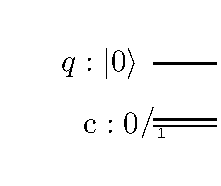
\includegraphics{Figures/Circuits/implementation/1zero.pdf}
\end{figure}

The default initial state is $\ket{0}$, but we can change initialize it to something else.

\begin{minted}{python}
    circuit.initialize(1, 0)
\end{minted}

Resulting in

\begin{figure}[H]
    \centering
    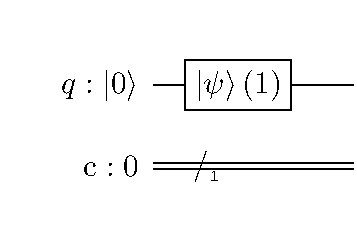
\includegraphics{Figures/Circuits/implementation/init1.pdf}
\end{figure}

We apply gates by specifying target qubit or qubits.

\begin{minted}{python}
     circuit.h(0) #Hadamard gate
\end{minted}

Which gives us

\begin{figure}[H]
    \centering
    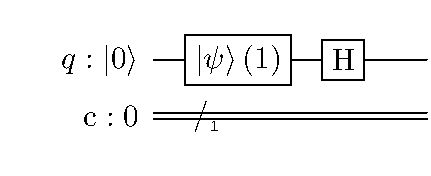
\includegraphics{Figures/Circuits/implementation/hada1.pdf}
\end{figure}

For controlled gates we add another qubit to the circuit:

\begin{minted}{python}
    quantum_reg = qk.QuantumRegistry(2)
    classical_reg = qk.ClassicalRegistry(2)
    circuit = qk.QuantumCircuit(quantum_reg, classical_reg)
    circuit.initialize(1, 0)
    circuit.h(0)
\end{minted}

Then a controlled gate is applied by specifying the control and target:

\begin{minted}{python}
    circuit.cx(0, 1) # Controlled Not gate
\end{minted}

And the result is

\begin{figure}[H]
    \centering
    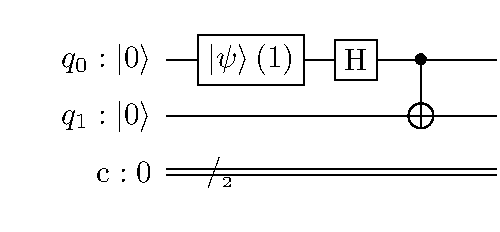
\includegraphics{Figures/Circuits/implementation/cx2.pdf}
\end{figure}


\section{Measurement and execution}

The measurement of a qubit is done by specifying the qubit to measure and which classical bit to store it into.

\begin{minted}{python}
    circuit.measure(0, 0)
    circuit.measure(1, 1)
\end{minted}

The circuit is then:

\begin{figure}[H]
    \centering
    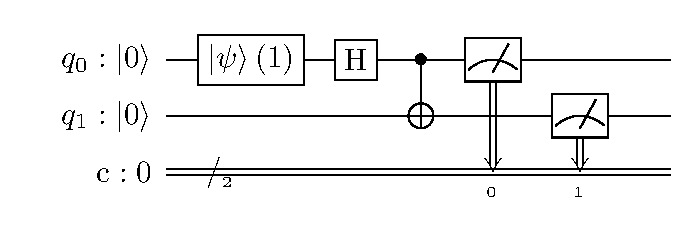
\includegraphics{Figures/Circuits/implementation/2measure.pdf}
\end{figure}

To run the code, or execute the circuit, we need to set up the backend. The backend is either a simulated quantum computer or a way for the program to communicate with a real one. Here we use the following simulator.

\begin{minted}{python}
    backend = qk.Aer.get_backend('qasm.simulator')
\end{minted}

Then we execute the circuit above.

\begin{minted}{python}
    job = backend.run(circuit, shots = 10_000)
\end{minted}

Where \textbf{shots} is how many times the circuit is to be run, as it is the average that is of interest. The results are then easily extracted.

\begin{minted}{python}
    counts = job.result().get_counts()
\end{minted}

Which is returned in the form of a dictionary.

\begin{minted}{python}
    counts = {
        '00' : n_00 #Number of |00> measured,
        '01' : n_01 #Number of |01> measured,
        '10' : n_10 #Number of |10> measured,
        '11' : n_11 #Number of |11> measured
    }
\end{minted}

\section{Copy and append}

The copy and append methods can speed up our code by reduce the number of times we need to add gates to a circuit. Say we have the circuit for the Y-basis transformation

\begin{minted}{python}
    quantum_reg = qk.QuantumRegistry(1)
    y_basis = qk.QuantumCircuit(quantum_reg)
    y_basis.sdg(0)
    y_basis.h(0)
\end{minted}

\begin{figure}[H]
    \centering
    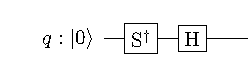
\includegraphics{Figures/Circuits/implementation/y-basis.pdf}
\end{figure}

and we want to append it to our previous circuit before measurements was added. We can then use qiskit's 'compose' method.

\begin{minted}{python}
     circuit.compose(y_basis, qubits = 0)
\end{minted}

And we get

\begin{figure}[H]
    \centering
    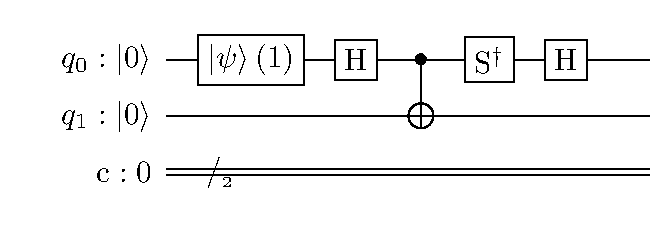
\includegraphics{Figures/Circuits/implementation/2mesy.pdf}.
\end{figure}

If we rather want to keep the base circuit for reuse, we can first create a copy and append to that one instead.

\begin{minted}{python}
    circuit_copy = circuit.copy()
    circuit_copy.append(y_basis, qubits = 0)
\end{minted}

